\section{Research Goals}

\begin{figure}
	\centering
	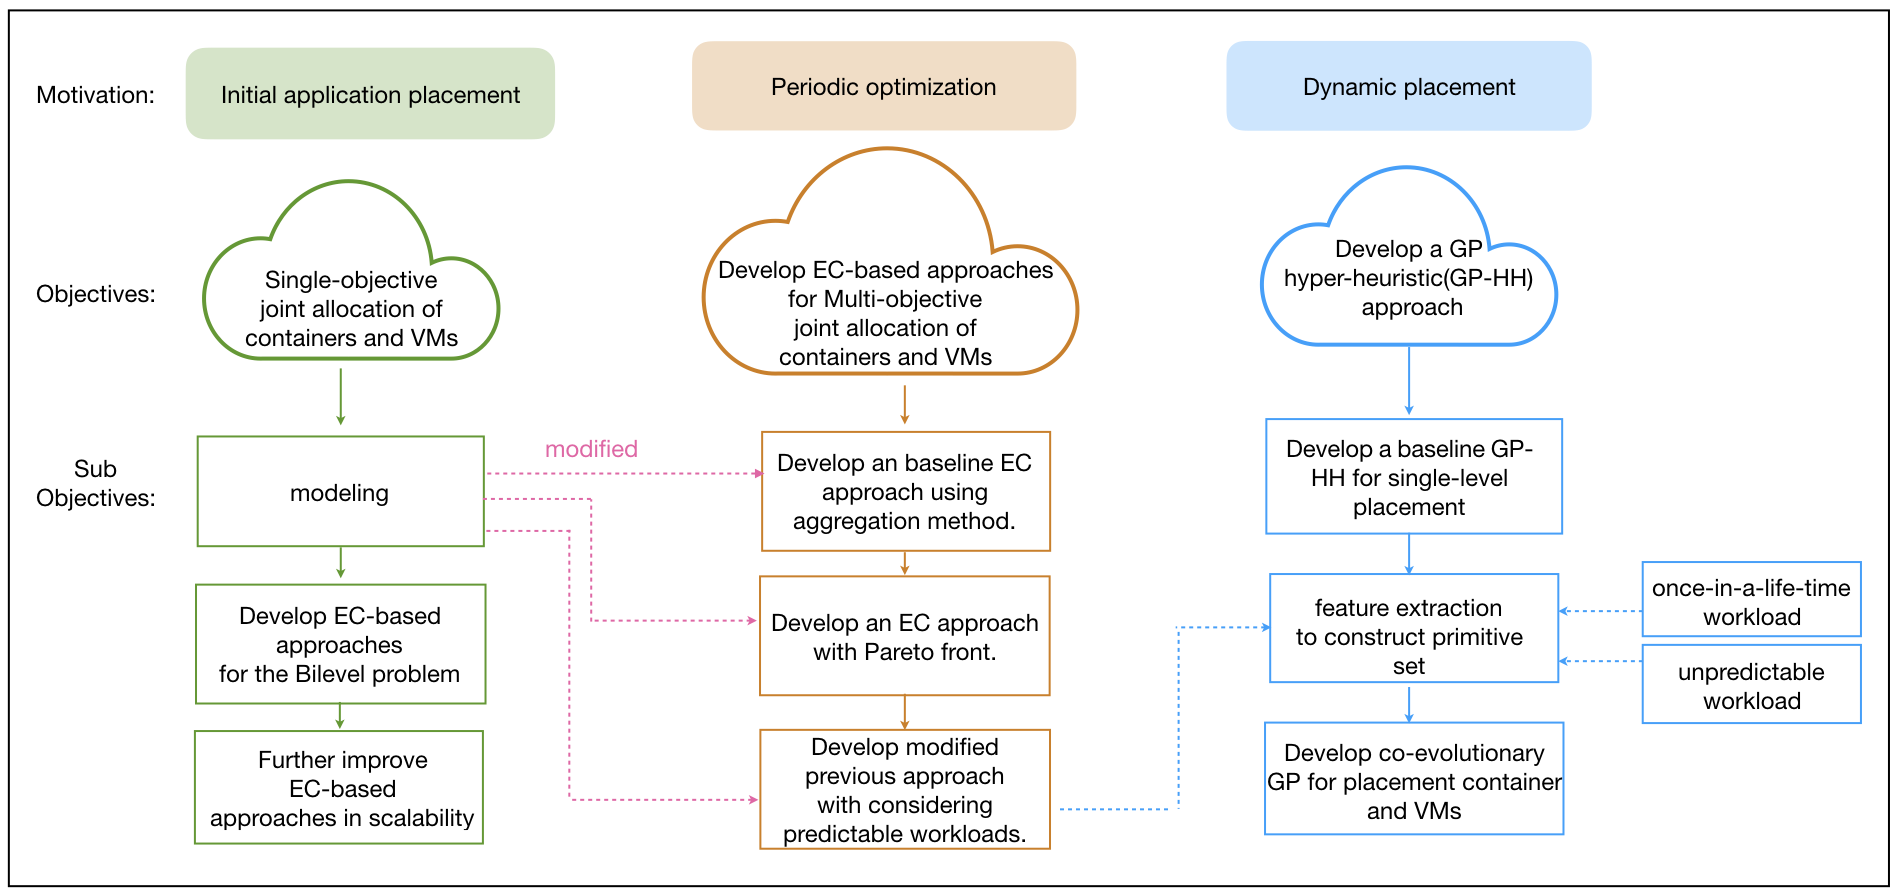
\includegraphics[width=\textwidth]{pics/thesisPlan.png}
	\caption{Relationship between objectives}
	\label{fig:objectives}
\end{figure}
\bx{The overall goal of this research is to optimize energy consumption of container-based clouds using EC-based approaches for three placement decision scenarios:} initial placement of applications, periodic placement of applications, and dynamic placement of applications. The specific research objectives of this work can be itemized as follows.
% In this thesis, we aims at providing a series of approaches to continuously optimize the joint allocation of VMs and containers that considers three consolidation scenarios: Initialization, global consolidation, Dynamic consolidation. In addition, the static allocation normally involves with large amount of variables which is particular difficult to optimize. We are also going to propose a method to solve this problem.  These approaches combine element of AI planning, to ensure the objectives and constraint fulfillment, and of Evolutionary Computation, to evolve a population of near-optimal solutions. The research aims at determining a flexible way in creation of solutions to solve server consolidation problems. As discussed in the previous section, the research goal can be achieved in the following objectives and sub-objectives.

\subsection{Objective One: Develop EC-based approaches for the single-objective joint placement of containers and VMs for initial placement of applications}
\label{sec:obj1}

\bx{The goal of objective one is to minimize energy consumption in initial placement of applications at container-based clouds.} We set three sub-objectives to achieve this goal. 
% The first sub-objective is to propose a new bilevel energy model for the joint placement of containers and VMs in PMs. The second sub-objective is to develop an EC-based optimization algorithm to solve the joint placement of containers and VMs. The third sub- objective improves scalability of the proposed EC-based optimization algorithm. 
For the sake of brevity and without loss of clarity, we will use ``the bilevel model/problem'' to replace ``the joint placement of containers and VMs model/problem'' in the following content. 
% \textcolor{Maroon}{Currently, most research on container consolidation do not consider the two-level of allocation problem.} Unlike previous VM-based service consolidation, 
% most research focus on VM-based server consolidation technique. They often modeled the VM allocation problem as a vector bin-packing problem \cite{Zhang:2016cx}. 
% Container adds an extra layer of abstraction on top of VM. The placement problem has become a two-step procedure, in the first step, containers are packed into VMs and then VMs are consolidated into physical machines. These two steps are inter-related to each other. Previous research \cite{Piraghaj:2015uf} solve this problem in separated steps where the first step allocates containers to VMs and the second step allocates VMs to PMs with simple bin-packing heuristics. According to Mann's \cite{Mann:2016hx} observation, these two allocations should be conducted simultaneously to reach a near-optima solution, which essentially minimizes the energy consumption.

\begin{enumerate}
	\item Sub-objective 1: Develop a new bilevel energy model to represent the relationship between five factors and energy consumption. The five factors involve locations of container, types of VM, locations of VM, overheads of VM, and the balance between memory and CPU. We need to consider the interaction between these factors.
	% \textcolor{Maroon}{This problem can be considered as a bilevel problem \cite{} the lower-level optimization: allocate containers to VMs and the upper-level: allocate VMs to PMs.} 
	% \textcolor{Maroon}{Since the existing models for container-based consolidation are based on VM-based model which incurs two problems.}
	% First problem is that they did not consider the interaction between two levels of allocation.
	% Second problem is that they did not consider balancing the residual resources (e.g between CPU and memory). 
	% \bx{The goal of the first sub-objective is to propose a bilevel model for the joint placement of container and VM.} 

	\bx{The major challenge of this sub-objective is that the bilevel energy model is more complicated than a single-level energy model.}
	\textbf{First}, in a VM-based model, the only factor is the locations of VMs in PMs. In contrast, in a container-based model,  the energy model involves four more variables. Specifically, locations of container decide the utilization of VMs. Types of VM constrain the placement of container. Overheads of VM bring extra workloads to the PMs. The balance of CPU and memory may indirectly impact on the energy consumption. Mishra \cite{Mishra:2011bz} finds better balance leads to a higher probability of allocating more applications. The above mentioned five factors are very likely to affect the energy consumption. \textbf{Second}, two pairs of interaction have not been considered. The first pair is the interaction between containers and types of VM. The second pair is the interaction between locations of container and locations of VM. Therefore, the bilevel energy model is very complicated.

	% Three challenges are listed as follows. \textbf{First}, the bilevel energy model is more complicated than a single-level energy model. The relationship among variables of the bilevel energy model has not been explored. In the VM-based energy model, the only variable is the location of VMs in PMs. In contrast,  container-based energy model has more variables such as the location of container, type of VM and the location of VM. \textbf{Second}, the balance of CPU and memory has an impact on the energy consumption  The more balance between CPU and memory in a PM, the higher probability of being able to allocate more applications. However, in container-based clouds, defining this balance is not straightforward because an additional variable of VM type has not been considered in previous study. \textbf{Third}, the overheads of VMs has not been considered in VM-based model because there is no better way to avoid the overheads. However, in container-based clouds, the overhead of VM can be mitigated by reducing the number of VMs. Therefore, adding the overhead of VM to the container-based energy model is necessary. 

	% The first issue is that it is still unclear that which energy function is the best to capture the relationship between container and VM so that the overall energy is low. Specifically, the objective for the lower level - placing container to VM, is still unclear. This is because the minimum number of VM does not necessary lead to the minimum number PMs; the types of VM also play an important role.
	% The second issue is that previous VM-based research do not consider the overhead of VM. However, the overhead of VMs is a major source of resource wastage (addressed in Section \ref{sec:comparison_container_vm}). Therefore, how to represent the impact of VMs remains unsolved.
	% The third issue is related to a VM-based research,  Mishra \cite{Mishra:2011bz} discovered that when multiple resources are considered in the model, the balance between resources has a heavy impact on the optimization results. Therefore, in the bilevel model, the balance of resources should also be considered.

	\bx{In order to establish a bilevel energy model, we propose to follow three steps and gradually add factors to the model. } Because the correlations between the five factors are complicated, we will study their correlation pair by pair. 
	\textbf{First}, we will consider the relationship between overheads, types of VM, and numbers of VM because they are closely related. In order to study the overheads of VM, we will review some research about VM hypervisors and study the impact of VMs. Our hypothesis is that the overheads have a linear relationship with the number of VMs and have no correlation with the type of VM. The outcome of the study of overheads will be a formulation that describes the relationship between overheads, types of VM, and numbers of VM.

	% We need to solve three open questions. 
	% \begin{enumerate}
	% 	\item How to represent the overhead of VM?
	% 	\item What is the correlation between overheads and types of VM?
	% 	\item What is the correlation between overheads and the number of VM?
	% \end{enumerate}
	% We expect to formulate the relationship between overheads, types of VM, and the number of VM. 
	\textbf{Second}, we will consider the balance between CPU and memory in both VM and PM levels. No one has yet considered the balance in the bilevel problem. We 
	will first consider formulating the balance in both levels. However, this formulation may have a high computation complexity. Hence, we will consider an aggregation of resources from both levels. Our hypothesis is that the aggregation can also achieve high utilization in PMs. The outcome of the study will be a formulation that describes the balance between CPU and memory in two levels.

	\textbf{Third}, we will consider the energy consumption with container, 
	VM, and PM. We will review some pieces of VM-based research \cite{Ferdaus:2014ep, Xu:2010vh, Gao:2013gg}. 
	The VM-based research generally represents resource demands as resource utilization. 
	We can use the similar idea to represent containers. The outcome of the study of overheads will be a formulation that describes the relationship between container, VM, PM, and energy consumption.
	% \begin{enumerate}
	% 	\item How to represent container, VM and PM?
	% 	\item What is the correlation between container and types of VM?
	% 	\item What is the correlation between the locations of container and VM?
	% \end{enumerate}
	
	\bx{This sub-objective 1 is expected, therefore, to formulate a bilevel energy model to represent the relationship between five factors.}

	% Each level of the problem will be formulated to a multi-dimensional vector bin packing problem. 
	% We will start from the simplest case - single dimension of resource - to more general multi-dimensional resources model by reviewing a number of VM-based approaches. Specifically, we focus on their variables, constraints and objective function. Objective function is mainly related to energy consumption. Hence, energy model is another major issue to study. In addition, in the multi-dimensional resource model, we will address the balance of CPU and memory problem by investigating several resource wastage models. In this objective, we consider the static workload of applications, this is because the initial resource demand is often provided by the Cloud users.


	% The novel contribution of this sub-objective is 


	\item Sub-objective 2: Propose a new EC-based bilevel optimization approach to solve the initial placement of applications to achieve better energy efficiency than VM-based approaches.\\
	% \bx{Based on the proposed bilevel model, the goal of this sub-objective is to develop an approach for the bilevel optimization problem using nested Evolutionary algorithms \cite{Sinha:2017et}.}

	\bx{We need to solve two challenges.} \textbf{The first challenge} is to design a representation of multiple variable types for EC-based optimization approach. Current VM-based representations only contain one type of variable while container-based representations contain three types of variables: locations of container, locations of VM and types of VM. Furthermore, current VM-based research generally applies binary representation (use 0 and 1 to represent placement). However, in container-based clouds, we cannot apply binary representation because it is not straightforward to represent bilevel of placement. 
	In addition, it is difficult to design a representation that narrows down the search space of solutions.  \textbf{The second challenge} is to design genetic operators and search mechanisms for an EC-based optimization approach. Since a bilevel optimization problem is known as a NP-hard problem \cite{Mathieu:2011dw}, the landscape of search space is ragged because of non-linearity, non-differentiability, non-convexity etc. Therefore, we need to further explore an effective search mechanism that can quickly locate feasible solutions.

	\bx{In order to solve the above challenges, we can learn from some existing approaches and design our bilevel approaches.} For the representation, we can review some VM-based research that uses direct discrete representation \cite{Xu:2010vh} and indirect continuous probability representation \cite{Xiong:2014jq}. We can learn from their approaches and then design our own such as the representation we design in preliminary work (Section \ref{sec:representation}). Furthermore, in order to quickly locate feasible solutions, we can embed a heuristic in the representation like in Section \ref{sec:representation}. 
	Based on our designed representation, we need to first investigate a few EC-based bilevel algorithms such as Genetic Algorithm (GA)-based approach: Cooperative coevolution algorithm \cite{Legillon:2012dd}, Particle Swarm Optimization (PSO)-based approach: Nested PSO \cite{Li:2006br} and others \cite{Angelo:2013ee, Zhu:2006in}. Then, we will choose an algorithm and design the genetic operators of the algorithm. For example, for GA-based algorithm, initialization operators should generate a diverse set of population and, ideally, the population contains feasible solutions. Mutation operator should allow the population to explore the entire solution space. Crossover operator creates better solutions based on the good genes in parents (previous good solutions).
	

	% In the bilevel problem, placing containers into a minimum number of VMs does not necessary lead to the minimum energy consumption. Therefore, it is still unclear that relation among the selection type of VM, placement of container and placement of VM will affect the energy consumption. Second challenge is how to design the search operators and representation. Currently two types of representation: direct and indirect representation can be considered. However, it is unclear that which one is more suitable for the nature of the bilevel problem. Third, bilevel optimization is strongly NP-hard , the solution space can be non-linearity, discreteness, no-differentiability, and non-convexity. Therefore, it is extremely difficult to design a proper search mechanism to find near optimal solutions.

	% In order to discover the relation among the selection type of VM, placement of container and placement of VM, we will first use one type of VMs and one type of container. By controlling these variables, the effect of different types of VMs and containers will be eliminated. Therefore, the relationship between bilevel placement would be clear. We will gradually add up variables and constraints. For the representation of bilevel problem, Genetic operators are also designed along with the proposed representation.

	\bx{We will evaluate our approaches in two ways.} \textbf{First}, in order to find the most suitable representation and EC-based algorithm, we will conduct experiments on different approaches and compare their performances in terms of energy efficiency. \textbf{Second}, we will compare our algorithm with existing VM-based approaches on the same benchmark dataset \cite{Shen:2015hm}. 

	\bx{This sub-objective 2 is expected to propose an EC-based approach for the initial placement of applications.} We expect this approach to achieve better energy efficiency than existing VM-based approaches \cite{Wilcox:2011ea, Xu:2010vh}.

	\item Sub-objective 3: Improve the scalability of the proposed EC-based approach a large number of applications.

	\bx{The major challenge of this task is the scalability of bilevel problems and the long computation time of EC-based approaches \cite{Sinha:2017et}.}

	\bx{We can use two methods: bottom-up and top-down to improve the scalability and decrease the computation time.} \textbf{First}, for the bottom-up method, we can reduce the number of variables by combining small containers
	into large combinations of containers. In the first step, we can use clustering approaches such as K-means \cite{Xie:2011fj} and decision tree to categorize containers into major groups and label them as ``CPU intensive'', ``Memory intensive'' etc. An open question is ``what kind of features should we use in clustering''.  In the second step, we will choose containers from these groups to construct combinations. An open question is ``what combination rule should we use''. Greedy-based rules may be useful to quickly construct combinations. In the third step is to decide the size of the constructed combination. Intuitively, large combinations (fewer variables) lead to lower computation complexity. On the other hand, larger combinations may lead to worse energy efficiency because the combinations are local. Therefore, a trade-off exists in computation complexity and energy efficiency. 

	\textbf{Second}, for the top-down method, we can separate a large problem into several sub-problems so that they can be executed in parallel. Similar to the bottom-up method, the top-down method also has a trade-off in computation complexity and energy efficiency. The divide-and-conquer approach is a top-down method.  After the divide-and-conquer approach splits a large problem into sub-problems, the smaller sub-problems are easy to solve individually. However, the aggregation of results from sub-problems may lead to local optima.  Therefore, we will investigate how to split the problem and the size of sub-problems. 

	\bx{We will evaluate our approach by comparing the energy efficiency and execution time with the previously proposed EC-based approach.}

	\bx{This sub-objective 3 is expected to improve the scalability of the previously proposed EC-based approach for up to one thousand applications without decreasing the energy efficiency.}


	% \bx{Three approaches can be potentially used in improving the scalability.} The first one is single-level reduction \cite{Sinha:2017et}, which reduces the bilevel problem into a single dimensional problem. Containers can be categorized into VMs which is then placed into PMs. The combination of container must be based on the knowledge of two-level placement interaction which we discover in the previous objective.  Then, complementary containers can be grouped to reduce the variables of placement. The challenge is to identify the features of static workload so that different workloads can be combined to fill a VM. Another way is use reinforcement learning to learn the pattern of energy-efficient combination of containers. 
	% The second approach is using a divide and conquer method to split the large number of containers into smaller chunks. The main challenge is that how to split the problem is unknown. Randomly dividing is very likely lead to a sub-optimal solution.
	% The third approach is combine heuristics into the EC algorithm, for example, develop a representation which is embedded with a simple heuristic (e.g First Fit). The heuristic is expected to reduce the search space so that the EC algorithm can find solution more efficiently. However, design a heuristic which embedded inside an EC algorithm is extreme difficult since evaluation of heuristic is indirect. 

	% \item Third, although nested approaches have been reported effective, they are often very time consuming. Therefore, our third sub-objective will focus on developing more efficient algorithms. There are several possible directions to be explored such as metamodeling-based methods \cite{Wang:2007em} and single-level reduction. 
		% \emph{New operators and searching mechanisms}\\
		% In order to utilize Evolutionary Computation (EC) to solve this problem, we are going to develop searching mechanisms according to the nature of problem as well as the selected representation. In order to achieve this goal, we will design several new operators. In order to evaluate the quality of these components, we will perform analytical analysis on the result.
\end{enumerate}
\subsection{Objective Two: Develop an EC-based approach for the multi-objective periodic placement of applications}
\bx{The goal of the second research objective is to develop a multi-objective EC-based approach for periodic placement of applications at container-based clouds with consideration of various types of workload.} The two objectives to be minimized are the energy consumption and the migration cost.
We set three sub-objectives to achieve this goal. 
% The first sub-objective proposes a multi-objective bilevel model for periodic placement of application taking into consideration with static workloads. The second sub-objective proposes an EC-based multi-objective algorithm with Pareto front approach. The third sub-objective extends the previous EC-based multi-objective algorithm to adapt to three types of workload: static, continuously increasing, and periodic.
% As previously (see Section  \ref{sec:motivation}) mentioned, the task is multi-objective: minimizing the number of migration and minimizing the overall energy consumption. This two objectives are conflicting since intensive optimization may incur a large number migration. The first challenge is how to solve the multi-objective bi-level optimization problem. In addition, we consider propose a robust periodic placement of application which means the placement of applications does not affect much from the variant workloads. Therefore, we divide workloads into five categories according to Fehling \cite{Fehling:2014tl}: static, periodic, once-in-a-life-time, continuously changing, and unpredictable. Among five types of workloads, two of them:  once-in-a-life-time and unpredictable workloads are unsuitable for static placement, since their behavior are hard to foresee and plan, hence, they are normally solved by dynamic approaches which will be addressed in our third objective.  For static, periodic, and continuously changing workload, we are going to design specific solutions. We also use three questions to guide our objective.
% The robustness of a data center is particularly important. 
% The robustness measures the stableness of result of consolidation.
% Furthermore, we will investigate proactive approaches - considering future allocation.
% In order to measure the degree of robustness, we need to design a robustness measure. The second sub-objective is to design static consolidation algorithm with considering its previous immediate result. The third objective extends the second objective to a more general case, considering both previous immediate and next allocation. The evaluation of algorithm is based on analytical analysis of fitness functions and robustness measure. 

\begin{enumerate}
	\item Sub-objective 1: Propose a multi-objective bilevel model for periodic placement with consideration of static workloads.  It has two objectives to be optimized: minimizing the energy consumption and minimizing the migration cost. \\

	\bx{The main challenge is that the migration model in container-based clouds is much complicated than the migration model in VM-based clouds.}
	\textbf{First}, in VM-based clouds, many research only considers the number of migrations \cite{Murtazaev:2014eo}. In container-based clouds, because the sizes of container vary in a wide range (e.g from MBs to GBs), it is inappropriate to simplify the migration cost as the number of migrations. Therefore, we will consider more factors such as network bandwidth to model the migration cost. This is a difficult task. \textbf{Second}, container-based migration model not only considers migration of VM, but also migration of container. Therefore, adding the migration model into our previous bilevel model is difficult. 

	\bx{In order to solve these challenges,} we will thoroughly study the differences of migration between VMs and containers. For example, VM contains an OS and all applications' data while containers only include data of an application. Then, we will explore some VM-based migration models that consider the size of VM and network bandwidth. We will consider to use a uniform model to represent the  cost of migrating VM and container.

	\bx{The sub-objective 1 is expected to formulate the bilevel model to represent both energy consumption and migration cost in container-based clouds.}

	% Because both container and VM can be migrated, it is unclear that migration model should be added to both layer or just one. One possible solution is to represent all VM migration with container migration. It may reduce the complexity. In addition, majority traditional migration models only consider the migration number without including the size of the applications which is unrealistic. Because the size will affect the overhead on the networking. 
	% The second challenge is to adapt the model to various types of workload. Previously, we simply the problem as applications can be represented as static workloads. In this sub-objective, we consider three types of predictable types of workload: static, linear continuous changing and periodic workload. These workloads may be represented as a function of time. Other models may also be changed accordingly.

	% We will further develop an EC-based multi-objective algorithm with aggregation approach to test the model. The aggregation approach turns a multi-objective problem into a single-objective problem by combining objectives into a single one. Therefore, we may use previous developed algorithm to solve periodic placement of application problem. We will use static workload to test the model. 

	\item Sub-objective 2: Propose a multi-objective bilevel EC-based algorithm for periodic placement of applications with Pareto front approach to achieve better performance than VM-based approach in both energy efficiency and migration cost.\\

	\bx{We need to solve three challenges.} \textbf{First}, the relationship between the two optimization objectives is very complicated. Since both migration cost and energy consumption can be non-convex, we cannot easily imagine the trade-off between two objectives. \textbf{Second}, we will design genetic operators to adapt the bilevel multi-objective optimization. Specifically, genetic operators in both levels collaborate with each other. Hence, it is more difficult to design the collaboration of operators between two levels.  \textbf{Third}, after obtaining a set of non-dominated solutions, we need to further design a fitness function assessment. The assessment selects one solution from a large number of non-dominated solutions based on some predefined preferences from Cloud providers. The selection of a solution can be a difficult task for a large size of non-dominated set \cite{Zio:2012jz}. 

	\bx{We will follow three steps to solve the above challenges.} \textbf{First}, to study the relationship between two objectives, we will first analyze the fitness functions of the objectives. For example, it is likely that in the migration function, the migration cost is monotonically increasing with the number of migrations and size of containers. After analyzing the fitness functions, we can visualize the relationship by using a technique called Trade-off region map \cite{Pinheiro:2015eu}. The trade-off region map can identify local and complex relationships between objectives, gaps in the fitness landscape, and regions of interest. \textbf{Second}, we will first choose an EC-based algorithm based on our previous experience from the objective one. Different from objective one, we will add trade-off control mechanisms such as non-dominated sorting into the genetic operators. \textbf{Third}, in order to design a fitness function assessment, we will review some priori and posteriori decision making support methods. On one hand, for priori methods, we assume Cloud providers have preferences according to the energy efficiency and migration cost.  On the other hand, for posteriori, we can design a clustering algorithm on the solution set and further narrow down solutions \cite{Zio:2011iq}. 
	 % such as Guided Multi-objective Genetic Algorithm \cite{Jat:2011us} and a clustering approach .

	\bx{We will evaluate our algorithm by comparing with existing VM-based approaches on the same benchmark dataset in terms of the energy consumption and migration cost.}

	\bx{This sub-objective 2 is expected to propose a multi-objective bilevel EC-based approach that can achieve better energy efficiency and migration cost than VM-based approaches.}

	% The major challenge in this sub-objective is to design genetic operators so that the proposed algorithm can steer the search close to the correct Pareto front. The aggregation approach proposed in previous sub-objective has some defects such as it cannot find the non-convex solution. A Pareto front approach is able to find a set of trade-off between objectives, therefore, we decide to explore this direction. Currently only a few research \cite{Yin:2000bt, Deb:2009jh,Deb:2010in} focus on bilevel optimization problem. This will be the first time that bilevel optimization with Pareto front approach is applied on a bilevel bin packing problem.
	% However, most of them are designed for continuous problems. Therefore, new representations and operators need to be considered for discrete problem. 

	% The assumptions for this objective, we will start from one dimensional of resource: CPU utilization. We will consider the static workload in this sub-objective because they are common and easy to start with.  We can utilize the representation and problem models from previous objective. However, we need to propose new genetic operators to adapt the multi-objective problem.

	% like the case in single objective problem, we need to develop new representations, genetic operators.
	\item Sub-objective 3: Extend the bilevel multi-objective algorithm for adapting three types of predictable workloads \cite{Fehling:2014tl}: static, linear continuously changing, and periodic. \\
	
	\bx{Several research mention the fluctuation of workloads has a heavy impact on  the periodic placement \cite{Verma:2009wi, Fehling:2014tl}.} Verma \cite{Verma:2009wi} states that treating workloads as static leads to a performance degradation of applications and low utilization of PMs. Verma considers three types of workloads: static, periodic, and unpredictable while Fehling \cite{Fehling:2014tl} considers three types of predictable workload: static, periodic and linear continuously changing, and two types of unpredictable workload: once-in-a-life-time and irregular. We believe Fehling's classification has a better coverage of existing workloads. Thus, we extend periodic placement on predictable workloads: static, periodic, and linear continuously changing to reach a more stable consolidation (less future migrations). Furthermore, because periodic and linear continuously changing workloads have distinct characteristics, for example, peak vs. no-peak, stable vs. unstable (constant mean value). Hence, we will study periodic and linear continuously changing workloads separately.

	\bx{To consider various types of workload, three challenges exist in this sub-objective.}
	First, it is difficult to reduce the dimensionality of raw workload dataset. Since a typical workload dataset may contain thousands of data point, the dimensionality reduction is critical before applying any similarity measure between workloads. Second, it is non-trivial to define the similarity between two workloads. The current measurement \cite{Verma:2009wi} only gives a correlation based on two workloads while we will measure the resource demand of an arbitrary number of workloads. Third challenge is to design representations and genetic operators to adapt to three types of workload.

	\bx{To tackle these challenges,} \textbf{first}, we can apply time-series analysis techniques on workloads such as Independent component analysis (ICA). ICA can extract features from large dimensionality of raw data so that three types of workload can be represented according to their features. \textbf{Then}, we can use a Pearson correlation to represent the similarity between two periodic workloads. \textbf{Third}, we will first try to design a uniform representation for all workloads so that all types of workload can be treated the same. However, if we cannot design a uniform representation, we may define a unique representation for each type of workload. Accordingly, we will design the genetic operators to suit the representations. 

	% Factor analysis such Principle Component Analysis \cite{Wold:1987wx} can be employed in developing new measure. Meanwhile, the representation used in static workload might not work, therefore, new representation, genetic operators need to be developed. 

	% Proactive consolidation \cite{Farahnakian:2015vj, Tan:2011jd} has driven a lot of attention in recent years. They mainly focus on making prediction of the workloads using a regression approach such as linear regression, multi-linear regression, and K-means regression. However, most of their consolidation methods are simple heuristics. In our approach, we seek to propose a combined technique.

	% \item Second, we will design a robustness measure. Previous studies only use simple measurement which counts the migration number between two static consolidation. This measurement aims at minimizing the number of migration between two  static placement processes. It may cause more migration in the next consolidation. Therefore, it needs a time-aware measure of the robustness of system. Therefore, in this objective, the first sub-problem we are going to solve is to propose a robustness measure. Currently, only a few research propose robustness aware server consolidation techniques \cite{Takouna:2014fa, Grimes:2016ia} have been proposed. They are either static threshold or probability-based threshold to measure the robustness of PMs. We will investigate an adaptive measure based on the historical data and current status.


	%  First, we need to design a new fitness function to measure the quality of the combination of various workload. 
	% \bx{The major challenge for this objective} According to the previously designed model, we will design representations for three types of workload. It is possible to design three distinct representations for three workloads. In addition, we must design search mechanisms to collaborate with the representations.

	\bx{The sub-objective 3 is expected to extend a multi-objective bilevel EC-based approach to three types of workload.}
	
	% \item \emph{Design a }\\

		% We will generalize the previous sub-objective to a more general one: design a time-aware allocation method which takes previous and next allocation into consider.
	\end{enumerate}




\subsection{Objective Three: Develop a hyper-heuristic single-objective Cooperative Genetic Programming Hyper-heuristic (GP-HH) approach for automatically generating dispatching rules for dynamic placement of applications.}

\bx{The goal of this objective is to develop a cooperative GP-based hyper-heuristic algorithm so that the generated dispatching rules can achieve both fast placement and global optimization with five types of workloads.} We set three sub-objectives to achieve this goal step by step. 
% The first sub-objective proposes a GP-based hyper-heuristic (GP-HH) algorithm for automatically generating dispatching rules for the single-level placement: container to VM with static workloads. The second sub-objective extracts features on the predictable workloads and two additional unpredictable workloads to construct a new primitive set. The third sub-objective develops a cooperative GP-HH approach for automatically generating dispatching rules for placing both containers and VMs.

% . 

% Therefore, in this objective, we will use GP to automatically generate heuristics or dispatching rules.

\begin{enumerate}

	\item Sub-objective 1: Develop a GP-based hyper-heuristic (GP-HH) algorithm for automatically generating dispatching rules for the single-level of placement:  VM to PM with static workloads. \\

	\bx{There are three reasons for us to develop a GP-HH for single-level placement.} \textbf{First}, previous dynamic consolidation methods, including both VM-based and container-based, are mostly based on bin-packing heuristics such as First Fit Descending. As Mann's research \cite{Mann:2015ua} shown, server consolidation is much harder than a bin-packing problem because of multi-dimensional of resources and many constraints. Therefore, general bin-packing algorithms do not perform well with many constraints and specific designed heuristics only perform well in a very narrow scope. \textbf{Second}, GP has been used in automatically generating dispatching rules in many areas such as job shop scheduling \cite{Nguyen:2014eu}. GP also has been successfully applied in bin-packing problems \cite{Burke:2006ei}. Therefore, we will investigate GP approaches for solving the dynamic consolidation problem. \textbf{Third}, we will first design a GP-HH for single-level of placement so that the two GP-HHs for bilevel of placement can cooperate.

	\bx{Two major challenges,} \textbf{first}, it is difficult to design a hyper-heuristics to generate dispatching rules. We will explore meaningful features of static workload, VM, and PM to construct a primitive set. It is uncertain that which feature can contribute to the dispatching rules.  \textbf{Second}, it is even difficult for the generated dispatching rules to reach a global optimal solution because of the trade-off between training accuracy and over-fitting.

	\bx{To gradually solve above challenges,} \textbf{first}, we start from reviewing the literature about manually designed heuristics and simple bin-packing heuristics. These heuristics contain some criteria, for example, First Fit algorithm normally considers the remaining resources of PM as the criteria of selecting a placement. We will also consider other features such as the status of VMs (e.g resource utilization), features of workloads (e.g resource requirement) that will affect the placement decision. The above features are represented as resource utilization. We will construct a primitive set with the selected features. 
	\textbf{Second}, we will use the default function set and the basic tree representation for constructing the dispatching rules. 
	\textbf{Third}, to train the GP-HH, we will use the solutions from the first objective as the learning sets. We can use ten folds cross-validation to prevent from over-fitting. 

	\bx{In order to evaluate the automatically generated heuristics, we will use a widely used simulator called CloudSim \cite{2009LNCS.5931...24B}.} Since our proposed algorithm is equivalent to a VM-based placement algorithm because they both focus on single-level of placement. We will compare our heuristic to a highly cited work \cite{Beloglazov:2012ji} from Beloglazov who proposes a Best Fit Decreasing heuristic for the energy consumption problem.

	\bx{The sub-objective 1 is expected to propose a GP-HH algorithm for automatically generating dispatching rules for the single-level placement with static workloads.} The generated dispatching rules are expected to achieve an equal or better performance than manually designed heuristics in terms of energy efficiency. 

	\item Sub-objective 2: Conduct feature extraction on the three predictable workloads and two unpredictable workloads to construct a new primitive set. \\
	
	\bx{The major challenge is to discover useful features that can represent various workloads.} The first challenge is to identify features from high dimensionality of datasets. The raw workload dataset may contain a large number of data points. It is difficult to extract meaningful features from the data points. The second challenge is to select useful features from a large number of raw features. It is very time consuming to manually examine raw features. The correlations between these raw features bring additional complexities.

	\bx{To solve these challenges, } \textbf{first}, we will review a number of dimensionality reduction techniques. Some possible techniques are sampling, extrema extraction. \textbf{Second}, we may employ the principle component analysis (PCA) technique on the feature set to reduce the number of features. 

	\bx{Classification of various workloads is one of the way to test the extracted features}. If we can differentiate workloads based on the extracted features with a high accuracy (e.g. 95\%), we can use the features to construct new dispatching rules. 

	\bx{The sub-objective 2 is expected to extract a number of features to represent different types of workload.} We can apply these features to construct a new primitive set so that the dispatching rules can deal with all kinds of workload.


	% types including static, continuously changing, and periodic workloads, and two other workload types: once-in-a-life-time, unpredictable workloads. Based on these features, 
	% \textcolor{Blue}{More...}
	% \item Investigate the possible functional operators. 

	% \bx{The goal of this sub-objective is to construct a GP functional set.}
	% \textcolor{blue}{More will come.}

	\item Sub-objective 3: Develop a cooperative GP-HH approach for automatically generating dispatching rules for placing both containers and VMs. \\
	\bx{The major challenge is to develop a cooperating procedure between two GP-HHs on two levels.} 
	As the first step, we will consider using two sub-populations to represent two-levels of placement. Each sub-population would be trained to minimize their objectives. The second step,the sub-population in the container-VM level will be used in training the VM-PM level of placement. 

	\bx{This sub-objective 3 is expected to propose a cooperative GP-HH approach for automatically generating dispatching rules for dynamic placement in container-based clouds.}

	% This sub-objective explores suitable representations for GP to construct useful dispatching rules. It also proposes new genetic operators as well as search mechanisms. \textcolor{blue}{More will come.}

	\end{enumerate}

% \subsection{Objective Four (Optional) Large-scale Static Consolidation Problem}
% Propose a preprocessing method to eliminate redundant variables 
% Current static consolidation takes all servers into consider which will lead to a scalability problem. In this objective, we will investigate two branches of methods, first one categorizes a number of containers into fewer groups so that the granularity decreases \cite{Piraghaj:2015uf}. Second method categorizes PMs so that only a small number of PMs are considered. This approach will dramatically reduce the search space. The potential approaches that can be applied in this task are various clustering methods.

	% The 
	% initial placement can be considered as a two-level of multi-dimensional bin-packing problem with multi-objectives. 
	% \item First, from the perspective of \emph{Cloud resource allocation model}, 
	% 	traditional Infrastructure as a Service (IaaS) resource allocation model 
	% 	considers service allocation and VM placement as separated responsibility.
	% 	Cloud users or brokers need to concern about the resource mapping and VM selection and 
	% 	Cloud providers take care of the VM placement. 
	% 	However, as Cloud users tend to over-provision in order to satisfy the QoS, they often book more
	% 	resources than their need. This is the major reason for the low utilization in 
	% 	Cloud computing \cite{Vogels:2008bg}. This problem cannot be 
	% 	resolved solely from the Cloud providers' perspective but to change the current resource allocation model. In the new resource allocation model, the responsibility of service allocation and VM placement are in the same hand of the Cloud provider.
	% 	Thereafter, Cloud providers have the full control of resource management. 
	% 	However, this process makes the VM initial placement a more complicated problem. Currently, only few researchers \cite{} have noticed this problem and propose initial work to address this problem.
	% \item Dynamic server consolidation is the process that the resource management continuously detects the server runtime status and if one of the server is overloaded. Then,
	% one of the VM or container running inside the server will be migrated to other machine 
	% so that the applications do not suffer from a performance degradation. In a container-based
	% environment, there are three questions to be answered. \emph{When to migrate ?} refers to determine the time point that a physical server is overloaded. \emph{Which container to migrate?} refers to determine
	% which container need to be migrated so that it optimize the global energy consumption.
	% \emph{Where to migrate?} refers to determine which VM and host that a container is migrated to.  
	% Specifically, in the second question, the main idea in the literature is still simple heuristics and random selection. Therefore, we are going to investigate using a genetic programming technique to learn to choose the best. In the 
	% third question, literature also rely on simple bin-packing heuristics which do not consider the impact of environment. Therefore, we are going to propose an idea which uses the features of workload, to decide which VM
	% is the best choice.

	% \item Static server consolidation is the process that a batch of VM and container joint is
	% consolidated in order to achieve an low energy consumption status. This stage is often
	% applied when the overall energy consumption is reached a predefine threshold. The static
	% server consolidation can globally optimize the energy consumption of the data center.
	% The process is similar with the initialization stage but with different objectives and constraints.

	% \item 

	% \item Second, container as a service has become an important trend in the 		Cloud computing industry and being support by many Cloud providers 	such as Amazon, Azure and many 
	% 	open-source projects. Both Cloud users and providers 
	% 	are beneficial to its lightweight. It provides a finer granularity resource management
	% 	for Cloud providers. From Ref \cite{}, we observed that VM-level consolidation could further improve the utilization of resource as well as the footprint from traditional hypervisors. 
	% 	However, there is not much container consolidation methods were discussed in the literature. 
	% 	New models and consolidation methods need to be proposed to solve the problem. Moreover, similar to
	% % 	VM placement, container placement is also an multi-objective which need to be addressed.

	% \item Third, the joint VM and container poses another level of consolidation problem. Ref \cite{} states, 
	% 	one of the reasons that container consolidation has high SLA violations is because the 
	% 	higher migration rate of containers. Therefore, designing algorithms that dynamically select between VM and container migration based on application SLA requirement as well as the impact on energy consumption is the major concern of the joint allocation. This can be treated as a dynamic task. 

	% \item Fourth, a common problem that faced by both traditional VM-based and the recent container-based data 	center is the affinity aware resource allocation problem. 
	% 	Modern Cloud-native applications normally have more than one copy of its implementation called replica in order to resolve the stateless as well as load balancing problem. Hence, they must be allocated into different servers to maintain its reliability. Similarly, the backup of databases has the same issue. In the CaaS scenario, more constraints appear such as operating system aware allocation which means, 
	% 	certain container can only be allocated in a specific operating system \cite{}. 
	% 	The affinity-aware allocation has been discussed in the literature, 
	% 	however, they can only be applied in the VM-based data center.   
	% \item Fifth, a resource-utilization aware co-location scheme can be helpful in order to resolve the 
	% 	resource competition problem. The study is about the behavior of the applications deployed
	% 	in the same physical machine. The previous research assumes that the applications' behavior
	% 	is a priori \cite{}, however, applications' behavior can be changed over time. It is important to allocate
	% 	the compatible applications in the same physical machine so that the physical machine reaches a 
	% 	stable status.

	% \item Sixth, large scale of server consolidation has always been a challenge in a Cloud data center. 
	% 	Especially, typical number of servers in a data center is at the million-level. Many approaches 
	% 	have been proposed in the literature to resolve the problem. 
	% 	There are mainly two ways, both rely on distributed methods, 
	% 	hierarchical-based \cite{} and agent-based management systems \cite{}.
	% 	The major problem in agent-based systems is that agents rely on heavy communication to maintain a high-level utilization. Therefore, it causes heavy load in the networking. Hierarchical-based approaches are the predominate methods. Hierarchical-based methods, in essence, are centralized systems where all the states of machines are collected and analyzed. One of way to improving the effectiveness of centralized system is to reduce the size of variables without losing too much of the consolidation performance. The main idea is to eliminating the high-utilized servers so that it reduces the dimensionality. 
% \end{enumerate}